\documentclass[journal,12pt,twocolumn]{IEEEtran}

\usepackage{setspace}
\usepackage{gensymb}
\singlespacing
\usepackage[cmex10]{amsmath}

\usepackage{amsthm}

\usepackage{mathrsfs}
\usepackage{txfonts}
\usepackage{stfloats}
\usepackage{bm}
\usepackage{cite}
\usepackage{cases}
\usepackage{subfig}

\usepackage{longtable}
\usepackage{multirow}

\usepackage{enumitem}
\usepackage{mathtools}
\usepackage{steinmetz}
\usepackage{tikz}
\usepackage{circuitikz}
\usepackage{verbatim}
\usepackage{tfrupee}
\usepackage[breaklinks=true]{hyperref}
\usepackage{graphicx}
\usepackage{tkz-euclide}

\usetikzlibrary{calc,math}
\usepackage{listings}
    \usepackage{color}                                            %%
    \usepackage{array}                                            %%
    \usepackage{longtable}                                        %%
    \usepackage{calc}                                             %%
    \usepackage{multirow}                                         %%
    \usepackage{hhline}                                           %%
    \usepackage{ifthen}                                           %%
    \usepackage{lscape}     
\usepackage{multicol}
\usepackage{chngcntr}

\DeclareMathOperator*{\Res}{Res}
\newtheorem{theorem}{Theorem}[section]
\newtheorem{corollary}{Corollary}[theorem]
\newtheorem{lemma}[theorem]{Lemma}
\newtheorem{definition}{Definition}[section]
\renewcommand\thesection{\arabic{section}}
\renewcommand\thesubsection{\thesection.\arabic{subsection}}
\renewcommand\thesubsubsection{\thesubsection.\arabic{subsubsection}}

\renewcommand\thesectiondis{\arabic{section}}
\renewcommand\thesubsectiondis{\thesectiondis.\arabic{subsection}}
\renewcommand\thesubsubsectiondis{\thesubsectiondis.\arabic{subsubsection}}


\hyphenation{op-tical net-works semi-conduc-tor}
\def\inputGnumericTable{}                                 %%

\lstset{
%language=C,
frame=single, 
breaklines=true,
columns=fullflexible
}
\begin{document}

\newcommand{\BEQA}{\begin{eqnarray}}
\newcommand{\EEQA}{\end{eqnarray}}
\newcommand{\define}{\stackrel{\triangle}{=}}
\bibliographystyle{IEEEtran}
\raggedbottom
\setlength{\parindent}{0pt}
\providecommand{\mbf}{\mathbf}
\providecommand{\pr}[1]{\ensuremath{\Pr\left(#1\right)}}
\providecommand{\qfunc}[1]{\ensuremath{Q\left(#1\right)}}
\providecommand{\sbrak}[1]{\ensuremath{{}\left[#1\right]}}
\providecommand{\lsbrak}[1]{\ensuremath{{}\left[#1\right.}}
\providecommand{\rsbrak}[1]{\ensuremath{{}\left.#1\right]}}
\providecommand{\brak}[1]{\ensuremath{\left(#1\right)}}
\providecommand{\lbrak}[1]{\ensuremath{\left(#1\right.}}
\providecommand{\rbrak}[1]{\ensuremath{\left.#1\right)}}
\providecommand{\cbrak}[1]{\ensuremath{\left\{#1\right\}}}
\providecommand{\lcbrak}[1]{\ensuremath{\left\{#1\right.}}
\providecommand{\rcbrak}[1]{\ensuremath{\left.#1\right\}}}
\theoremstyle{remark}
\newtheorem{rem}{Remark}
\newtheorem*{remark}{Remark}
\newcommand{\sgn}{\mathop{\mathrm{sgn}}}
\providecommand{\abs}[1]{\vert#1\vert}
\providecommand{\res}[1]{\Res\displaylimits_{#1}} 
\providecommand{\norm}[1]{\lVert#1\rVert}
%\providecommand{\norm}[1]{\lVert#1\rVert}
\providecommand{\mtx}[1]{\mathbf{#1}}
\providecommand{\mean}[1]{E[ #1 ]}
\providecommand{\fourier}{\overset{\mathcal{F}}{ \rightleftharpoons}}
%\providecommand{\hilbert}{\overset{\mathcal{H}}{ \rightleftharpoons}}
\providecommand{\system}{\overset{\mathcal{H}}{ \longleftrightarrow}}
	%\newcommand{\solution}[2]{\textbf{Solution:}{#1}}
\newcommand{\solution}{\noindent \textbf{Solution: }}
\newcommand{\cosec}{\,\text{cosec}\,}
\providecommand{\dec}[2]{\ensuremath{\overset{#1}{\underset{#2}{\gtrless}}}}
\newcommand{\myvec}[1]{\ensuremath{\begin{pmatrix}#1\end{pmatrix}}}
\newcommand{\mydet}[1]{\ensuremath{\begin{vmatrix}#1\end{vmatrix}}}
\numberwithin{equation}{subsection}
\makeatletter
\@addtoreset{figure}{problem}
\makeatother
\let\StandardTheFigure\thefigure
\let\vec\mathbf
\renewcommand{\thefigure}{\theproblem}
\def\putbox#1#2#3{\makebox[0in][l]{\makebox[#1][l]{}\raisebox{\baselineskip}[0in][0in]{\raisebox{#2}[0in][0in]{#3}}}}
     \def\rightbox#1{\makebox[0in][r]{#1}}
     \def\centbox#1{\makebox[0in]{#1}}
     \def\topbox#1{\raisebox{-\baselineskip}[0in][0in]{#1}}
     \def\midbox#1{\raisebox{-0.5\baselineskip}[0in][0in]{#1}}
\vspace{3cm}
\title{Gate Assignment 4}
\author{Yashas Tadikamalla - AI20BTECH11027}
\maketitle
\newpage
\bigskip
\renewcommand{\thefigure}{\theenumi}
\renewcommand{\thetable}{\theenumi}
Download all python codes from 
\begin{lstlisting}
https://github.com/YashasTadikamalla/EE3900/blob/main/GateAssignment4/codes
\end{lstlisting}
%
and latex-tikz codes from 
%
\begin{lstlisting}
https://github.com/YashasTadikamalla/EE3900/blob/main/GateAssignment4/GateAssignment4.tex
\end{lstlisting}
\section{Problem (EC-1997 Q1.10)}
A deterministic signal has the power spectrum given in the figure. The minimum sampling rate needed to completely represent this signal is
\begin{figure}[!h]
 \centering
 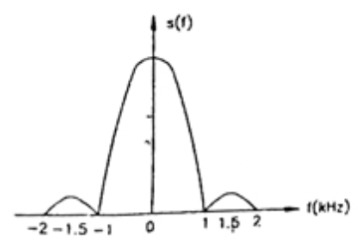
\includegraphics[width=\columnwidth]{GateAssignment4.jpeg}
 \label{plot}
\end{figure}
\begin{enumerate}
    \item $1 KHz$
    \item $2 KHz$
    \item $3 KHz$
    \item None
\end{enumerate}
\section{Solution}
\begin{definition}[Normalised sinc function]
A normalised sinc function is defined as
\begin{align}
    sinc(x)=\begin{cases}
	1, & x=0 \\~\\[-1em]
	\dfrac{sin(\pi x)}{\pi x}, & x\neq 0
	\end{cases}
	\label{eq:sinc}
\end{align}
\end{definition}
\begin{definition}[Power spectrum]
Power Spectral density, or simply, Power spectrum, denoted by $s(f)$ is defined as  \label{eq:def}
\begin{align}
    s(f)=\abs{X(f)}^2
\end{align}
\end{definition}
\begin{theorem}[Sampling Theorem]
If a signal contains no frequency components above W Hz, then the sampling rate at which the continuous time signal needs to be sampled uniformly, so as to completely recover the original signal is given by\label{samp}
\begin{align}
    f_s\geq2W
    \label{eq:sthm}
\end{align}
\end{theorem}
\begin{definition}[Nyquist rate]
Minimum sampling rate is also called as Nyquist rate. It is given by
\begin{align}
    f_s=2W
    \label{eq:ns}
\end{align}
\end{definition}

Given, power spectrum of a deterministic signal. From \eqref{eq:def}, Fourier transform of the given band limited signal is \textbf{truncated normalised sinc pulse}. As no frequency component exceeds $2 KHz$,
\begin{align}
    W=2 KHz
\end{align}
From \eqref{eq:ns}, 
\begin{align}
    f_s&=2W=4 KHz
\end{align}
Hence, option 4 is the correct answer.


To verify the validity of \eqref{samp}, let's see what happens if we sample at a rate lower than Nyquist rate.

Let our original continuous time signal be $x(t)$. Consider impulse train $x_i(t)$ given by
\begin{align}
    x_i(t)=\displaystyle\sum_{n=-\infty}^{\infty}\delta(t-nT_s)
\end{align}
where $T_s$ is the sampling period. ($f_s=\dfrac{1}{T_s}$ is the sampling frequency). The sampled signal would be
\begin{align}
    x_s(t)&=x(t)x_i(t)\label{eq:temp}\\
    &=\displaystyle\sum_{n=-\infty}^{\infty}x(nT_s)\delta(t-nT_s)
\end{align}
Also, from \eqref{eq:temp}
\begin{align}
    X_s(f)&=X(f)*X_i(f)\\
    &=\dfrac{1}{T_s}\displaystyle\sum_{k=-\infty}^{\infty}X(f-kf_s)
\end{align}
$X_s(f)$ consists periodically repeated copies of $X(f)$, shifted by integer multiples of $f_s$. For our example, $X(f)$ is the \textbf{truncated normalised sinc pulse}. Let $W$ be the the maximum frequency component. 
\begin{figure}[!h]
 \centering
 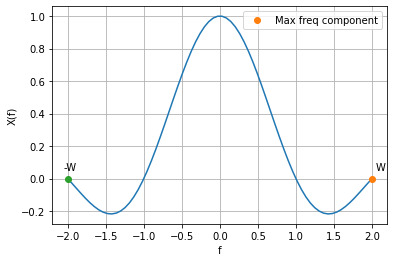
\includegraphics[width=\columnwidth]{GateAssignment4(1).png}
 \caption{Plot of X(f)}
 \label{plot}
 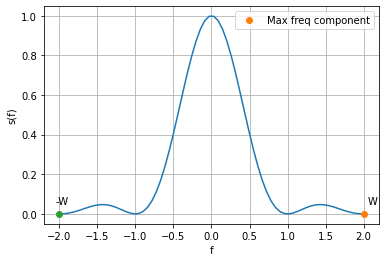
\includegraphics[width=\columnwidth]{GateAssignment4(2).png}
 \caption{Plot of s(f)}
 \label{plot}
\end{figure}
\begin{itemize}
    \item Case 1: $W>2f_s$: 
    
    The copies don't overlap. Hence, $x(t)$ can be recovered from $x_s(t)$ using a low pass filter.
    \item Case 2: $W=2f_s$: 
    
    The copies just touch each other, but don't overlap. So, $x(t)$ can be recovered from $x_s(t)$ using a low pass filter.
    \item Case 3: $W<2f_s$:
    
    As the copies overlap, they get added. So, we cannot reconstruct the original signal $x(t)$. This gives rise to situation called aliasing.
\end{itemize}
\begin{figure}[!h]
 \centering
 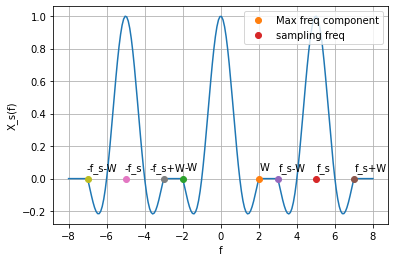
\includegraphics[width=\columnwidth]{GateAssignment4(3).png}
 \caption{$W>2f_s$}
 \label{plot}
 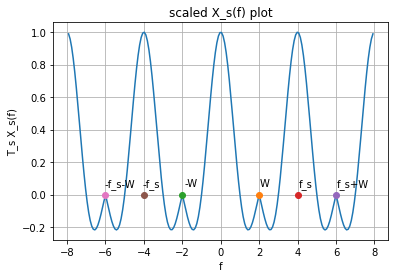
\includegraphics[width=\columnwidth]{GateAssignment4(4).png}
 \caption{$W=2f_s$}
 \label{plot}
 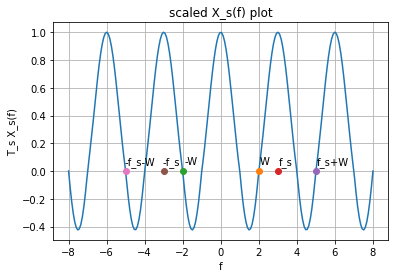
\includegraphics[width=\columnwidth]{GateAssignment4(5).png}
 \caption{$W<2f_s$}
 \label{plot}
\end{figure}

Hence, we need to sample at a rate greater than Nyquist rate to be able to recover the original signal.
\end{document}



